
\documentclass[article]{standalone}
\usepackage{tikz}

\begin{document}
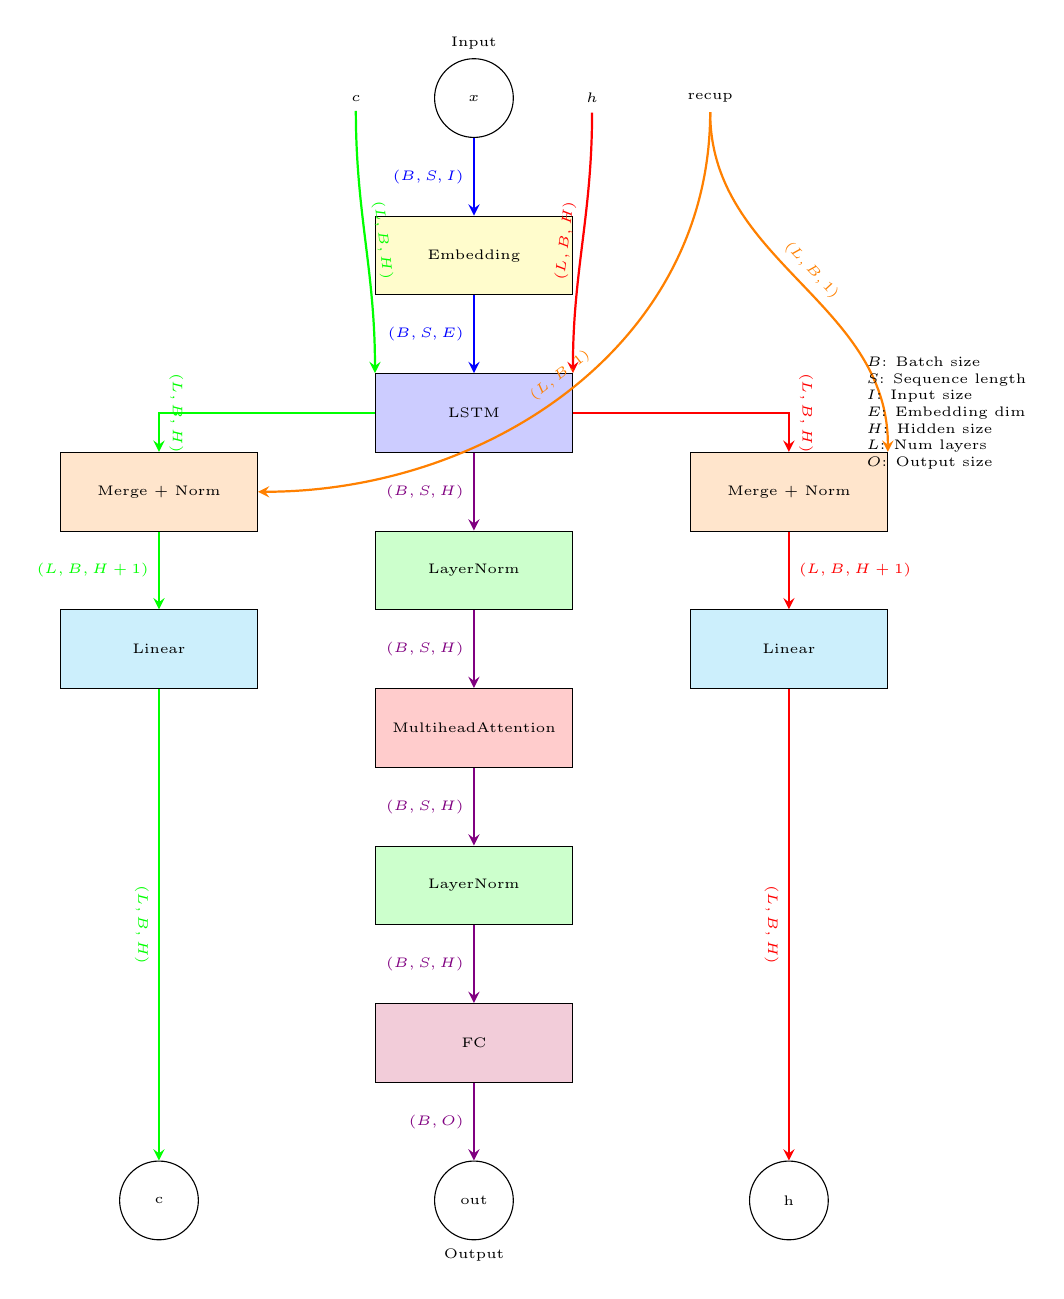
\begin{tikzpicture}[
  box/.style={draw, rectangle, minimum width=2.5cm, minimum height=1cm},
  input/.style={draw, circle, minimum size=1cm},
  arrow/.style={->, >=stealth, thick},
  every node/.style={font=\tiny}
]

% Input
\node[input] (x) at (0,0) {$x$};
\node[left of=x, node distance=1.5cm] (c) {$c$};
\node[right of=x, node distance=1.5cm] (h) {$h$};
\node[right of=h, node distance=1.5cm] (recup) {recup};

% Embedding
\node[box, fill=yellow!20] (emb) at (0,-2) {Embedding};

% LSTM
\node[box, fill=blue!20] (lstm) at (0,-4) {LSTM};

% Layer Norm
\node[box, fill=green!20] (norm1) at (0,-6) {LayerNorm};

% Attention
\node[box, fill=red!20] (attn) at (0,-8) {MultiheadAttention};

% Layer Norm
\node[box, fill=green!20] (norm2) at (0,-10) {LayerNorm};

% Fully Connected
\node[box, fill=purple!20] (fc) at (0,-12) {FC};

% Output
\node[input] (out) at (0,-14) {out};
\node[input] (c_out) at (-4,-14) {c};
\node[input] (h_out) at (4,-14) {h};

% Hidden state processing
\node[box, fill=orange!20] (norm_h) at (4,-5) {Merge + Norm};
\node[box, fill=cyan!20] (h_fc) at (4,-7) {Linear};

% Cell state processing
\node[box, fill=orange!20] (norm_c) at (-4,-5) {Merge + Norm};
\node[box, fill=cyan!20] (c_fc) at (-4,-7) {Linear};

% Connections
\draw[arrow, blue] (x) -- node[left] {$(B,S,I)$} (emb);
\draw[arrow, blue] (emb) -- node[left] {$(B,S,E)$} (lstm.north);
\draw[arrow, violet] (lstm.south) -- node[left] {$(B,S,H)$} (norm1);
\draw[arrow, violet] (norm1) -- node[left] {$(B,S,H)$} (attn);
\draw[arrow, violet] (attn) -- node[left] {$(B,S,H)$} (norm2);
\draw[arrow, violet] (norm2) -- node[left] {$(B,S,H)$} (fc);
\draw[arrow, violet] (fc) -- node[left] {$(B,O)$} (out);

\draw[arrow, red] (h) to[out=-90,in=90] node[above, sloped] {$(L,B,H)$} (lstm.north east);
\draw[arrow, green] (c) to[out=-90,in=90] node[above, sloped] {$(L,B,H)$} (lstm.north west);
\draw[arrow, orange] (recup) to[out=-90,in=90] node[above, sloped] {$(L,B,1)$} (norm_h.north east);
\draw[arrow, orange] (recup) to[out=-90,in=0] node[above, sloped] {$(L,B,1)$} (norm_c.east);


\draw[arrow, red] (lstm.east) -| node[above, sloped] {$(L,B,H)$} (norm_h);
\draw[arrow, red] (norm_h) -- node[right] {$(L,B,H+1)$} (h_fc);
\draw[arrow, red] (h_fc) to[out=-90,in=90] node[below, sloped] {$(L,B,H)$} (h_out);

\draw[arrow, green] (lstm.west) -| node[above, sloped] {$(L,B,H)$} (norm_c);
\draw[arrow, green] (norm_c) -- node[left] {$(L,B,H+1)$} (c_fc);
\draw[arrow, green] (c_fc) to[out=-90,in=90] node[below, sloped] {$(L,B,H)$} (c_out);

% Input labels
\node[above of=x, node distance=0.7cm] {Input};
\node[below of=out, node distance=0.7cm] {Output};

% Legend
\node[right of=lstm, node distance=6cm, align=left] {
$B$: Batch size \\
$S$: Sequence length \\
$I$: Input size \\
$E$: Embedding dim \\
$H$: Hidden size \\
$L$: Num layers \\
$O$: Output size
};

\end{tikzpicture}

\end{document}